\chapter{Deployment of the distributed enumeration project}
% put these two lines after every \chapter{} command
\vspace{-2em}
\minitoc

Chapter 5 will contain details pertaining to the method of deploying a small-scale distributed search based on the design set out in Chapter 4 as a proof of concept.  It will include how awareness of the project was raised in the scientific community, the  challenges involved in launching the project as well as the lessons learnt for the possible future deployment of larger scale projects.  The chapter will conclude with the results of the distributed computing project designed in Chapter 4, most likely the enumeration of main classes of MOLS of order 8 or 9.  It will also give a summary of the distributed enumeration in terms of number of volunteers, locality, how work was done by each of the volunteers etc. 

\section{Creating a volunteer computing project for the enumeration of 3-MOLS of order 8}
\subsection{Server architecture} \label{5server}
An initial BOINC server was set up inside a virtual machine running the Debian 6 operating system with 8Gb virtual hard disk and dedicated access to 384Mb random access memory (RAM) from the host. The machine hosting the virtual machine has a 64-bit Linux distribution with 8Gb of RAM. 
The virtual machine is run with \emph{bridged ethernet}, which means that it shows up as a separate machine on the network with its own static IP address so that the server is always available at the same address for both volunteers signing up and hosts communicating with the server.
\subsection{Grid-enabling the exhaustive enumeration algorithm} \label{5grid}
The exhaustive enumeration of sets of $k$ mutually orthogonal \lat s, as described in \S\ref{Menum}, parallelises trivially - the subtrees rooted at  the nodes of level $i$, for any level $i$, may be enumerated completely independently. The   number of branches on the respective levels of the subtree  rooted at $\p$ level $i-1$ is simply the sum of the branches counted on every level in the respective enumerations of the children (on level $i$) of node $\p$.

The main modification required to grid-enable the   enumeration of MOLS is the addition of checkpointing. As described in \S\ref{Bapi}, the main goal of letting an application checkpoint, or save the current state of the computation in such a way that the computation may be restarted from it without any loss in accuracy, is to guard against losing progress through unpredictable volunteer and host behaviour. An application which takes 24 hours of computing to complete a workunit, does not checkpoint and runs on a host which is only available between 08:00 and 17:00, for example, would never return results since 9 hours of computations are lost every day when the computer is switched off. The enumeration algorithm lends itself to checkpointing, since, once $u_i(j)$ has been fixed for all values of $i$ up to some integer $m$, the number of feasible candidate universals for $u_{m+1}(j)$, prior to checking for orthogonality and class representatives, is completely deterministic. Indeed, the   list of candidate universals for $u_{m+1}(j)$ are always generated in exactly the same order, which means that any partial \lat \ may be described by giving the position in the list of candidate universals of the universal selected. 
All that is required to represent a partially filled MOLS, and therefore any node of the original search tree, in this manner is the positions of the selected universals in each of the \lat s, since the squares are completely independent prior to the test for orthogonality.

To be able to restart the enumeration from a checkpoint, the original algorithm was adapted so that, after reading the initial partial MOLS from an input file, it would search for a checkpoint file and, if one is available,  read the   numbers of previously counted branches. 
The enumeration then starts at the designated candidate universals instead of the first candidate universal generated. Care was taken to ensure that branches which were counted prior to checkpointing are not  counted twice, although some branches are enumerated a second time in  returning the computation to its previous state. 
Figure \ref{fig:checkpoint} shows how the  traversal of a hypothetical search tree would checkpoint. 
The branches in blue were counted   before checkpointing and is not revisited, while the purple branches were also counted before checkpointing but is traversed twice since they have to be visited again in order to return the search to its previous position. 
The red branches remain to be counted once the the traversal restarts from the checkpoint.\begin{wrapfigure}{r}{10cm}
\centering
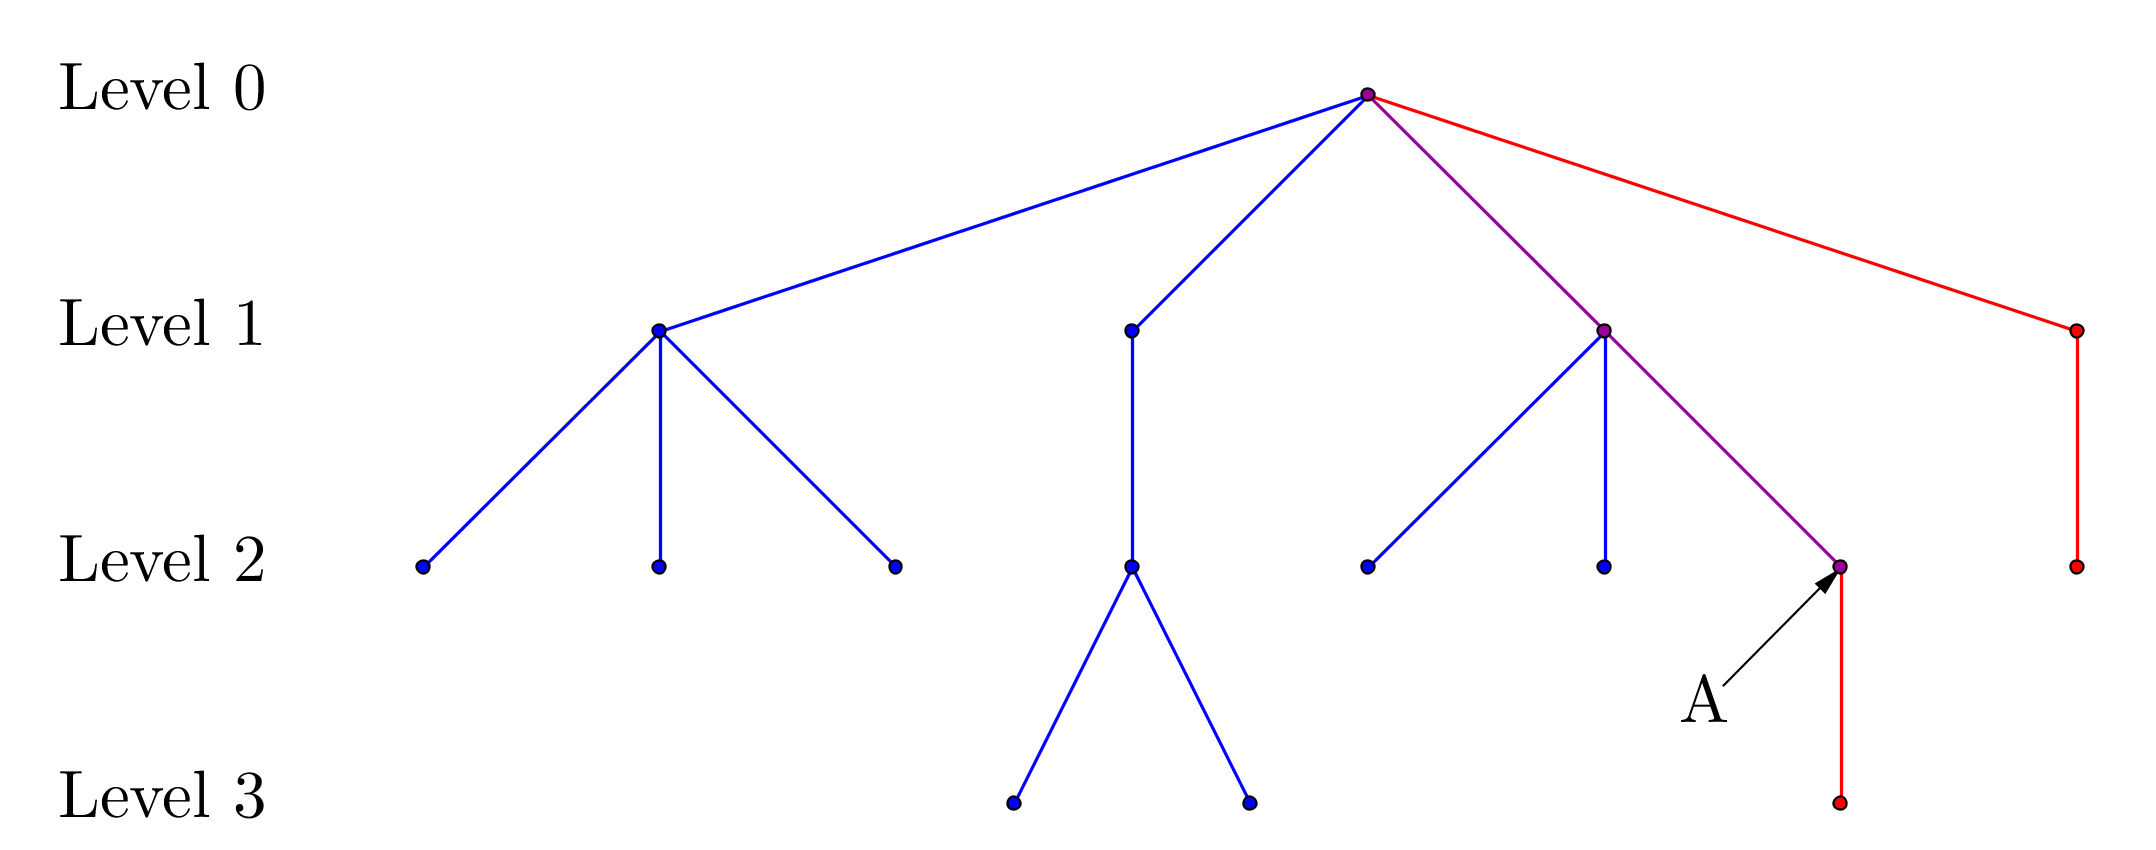
\includegraphics[width=10cm]{images/checkpointing2}
\caption{A  hypothetical enumeration tree showing the checkpointing strategy. The blue part of the tree is traversed prior to checkpointing at the node labelled A, the purple part of the tree is traversed both prior to checkpointing and when restarting from the checkpoint, and the red portion will be traversed after restarting from the checkpoint at A.} \label{fig:checkpoint}
\end{wrapfigure} 
In this case the checkpoint file   will   store  that the current node  at the time of checkpointing (labelled A in Figure \ref{fig:checkpoint}) may be reached by choosing child three of four on the first level and child three from three on the second, and that the traversal has encountered 1 node  on level 0 thusfar, 3 on level 1, and 7 and 2 on levels 2  and 3, respectively. 
The checkpoint   also registers the time that a computation has taken to date so that the   enumeration time  reported upon completion reflects the  actual total computation time. A new checkpoint  replaces all older ones so that there is always at most  one checkpoint available, thereby ensuring that the application restarts in its most recent location.

A final modification required to the application was to let it read input files from the logical file  'in', write results to the logical file  'out' and read and write checkpoints to the logical file 'state.' Recall from \S\ref{Bapi} that the result template, along with the BOINC API call \verb|boinc_resolve_filename()|, may be used to convert logical names to actual file names for every individual result.

\subsection{Deamons} \label{5deamons}
Deamons were tasked with performing actions on the server as described in \S\ref{Bapi}. Work generation takes places with a bash\footnote{See \cite{bash} for more information on the bash shell} script which loops through the forty-five partial MOLS found after inserting the 0-universals into each of the three squares and creates a corresponding workunit in the project database with an estimated runtime of $10^{14}$ floating-point operations, or approximately 720 hours, and a delay bound of 10 days before the scheduler gives up on a dispatched result.

Replication was used to ensure the correctness of the returned results, two results were initially created for every workunit and the quorum was set to 2. Results are validated with a custom validator which compares the number of branches found on every level of the tree. It was not possible to use the sample bitwise generator since the enumeration time, which may differ between different hosts, is also included in the result.
The default scheduler and sample assimilator may, however, be used, since post-processing only consists of moving the results to a specific folder, which is exactly what the the sample assimilator does. 

\subsection{Preliminary enumeration results} \label{5pres}
The 3-MOLS of order 10 were enumerated through a BOINC project on five hosts of the same platform, specifically Intel processors with  a Linux distribution.



%\begin{table}[ htb]
% \centering \vspace{-.2cm}\caption{The number of errors (E), valid (V) and invalid (I) results computed by each of the hosts, as well as the credit granted and complete enumeration time in the enumeration of 3-MOLS of order 8.}\vspace*{-.2cm}
%\begin{tabular}{lrrrrrrrrrr}
%\toprule
%Host & Errors & Valid & Invalid & Credits  & CPU Time \\
%$1$ & $4$ & $2$ & $0$ & $1027.64$ & $211469.7$ & $70273.14$ & $70317.79$ & $105734.85$ \\
%$3$ & $1$ & $36$ & $2$ & $4969.13$ & $730630.1$ & $1.76$ & $133338.00$ & $20295.28$ \\
%$4$ & $29$ & $43$ & $0$ & $6104.15$ & $1621431.3$ & $11.12$ & $78548.30$ & $37707.70$ \\
%$5$ & $8$ & $14$ & $0$ & $10488.90$ & $1352450.0$ & $47517.09$ & $104348.50$ & $96603.57$ \\
%$6$ & $2$ & $7$ & $0$ & $5566.54$ & $713200.4$ & $84747.34$ & $111181.80$ & $101885.76$ \\
%$Total$ & $44$ & $102$ & $2$ & $28156.36$& $4629181.4$\\
%
% \bottomrule
%\end{tabular}\vspace*{.1cm}
%\label{83naivehosts}
%\end{table}
  \begin{table}[htb]
 \centering
 \caption{The number of results issued in each section of the enumeration tree during the distributed enumeration of 3-MOLS of order 8, along with the resulting redundancy.}
\begin{tabular}{lrrrrrrr}
\toprule
Section & Nodes on    & Workunits & \multicolumn{4}{c}{Results} & Redundancy  \\
\cmidrule(lr){4-7}
 &level 0 && Validated & Error  & Invalid & Total &($r$)      \\ \midrule 
$z_1z_2^2z_3$ & 17& 23&46&43& 0& 89&$5.2$  \\ 
$z_1z_2^1z_5$ &14&14&28&1& 2&31&$2.2$   \\ 
$z_1z_3z_4$& 5&5&10&0&0&10& $2$    \\ 
$z_1z_7$ & 9&9&18&0&0&18&$2$   \\ \midrule
Total &45 &51&102&44&2&142&$3.3$   \\ \bottomrule
\end{tabular}\vspace*{.4cm}
\label{83naivesumm}
\end{table} 
A summary of the enumeration is presented in Tables  \ref{83naivesumm}--\ref{83naivebranches}. Table \ref{83naivesumm} shows the total number of results dispatched to hosts, along with the number of validated, invalid and erroneous results received.
 There was a particularly high error rate in the first section of the enumeration tree, where six of the workunits exceeded their maximum number of allowable errors (in this case 3) and had to be recreated. These errors played a large part increasing the overall redundancy rate from 2 to 3.2 and need to be investigated prior to further enumeration attempts.  The total number of erroneous, valid and invalid results may be seen in Table \ref{83naivehosts}, along with the total credit granted to each host for valid results and the total time that the computations took.
 \begin{wraptable}{r}{8.2cm}
 \centering \vspace{-.2cm}\caption{The number of errors (E), valid (V) and invalid (I) results computed by each of the hosts, as well as the credit granted and complete enumeration time in the enumeration of 3-MOLS of order 8.}\vspace*{-.2cm}
\begin{tabular}{lrrrrrrrrrr}
\toprule
Host & E & V & I & Credit  & CPU Time \\ \midrule
$1$ & $4$ & $2$ & $0$ & $1\,027.64$ & $211\,469.7$ \\
$3$ & $1$ & $36$ & $2$ & $4\,969.13$ & $730\,630.1$ \\
$4$ & $29$ & $43$ & $0$ & $6\,104.15$ & $1\,621\,431.3$ \\
$5$ & $8$ & $14$ & $0$ & $10\,488.90$ & $1\,352\,450.0$ \\
$6$ & $2$ & $7$ & $0$ & $5\,566.54$ & $713\,200.4$ \\ \midrule
  & $44$ & $102$ & $2$ & $28\,156.36$& $4\,629\,181.4$\\
 \bottomrule
\end{tabular}\vspace*{.1cm}
\label{83naivehosts}
\end{wraptable} 
 Note that the host with the identification number 2 did not connect to the project during this enumeration and is thus excluded from the summary.   
 It is clear from Table \ref{83naivehosts} that the majority of the errors occurred on   host 4 and closer inspection showed that this was due to incorrect client setup on that host. The total enumeration time increased by a factor of approximately 5 from the enumeration in \S\ref{Menum}. This increase is considerably more than the overall redundancy of 3.2 would suggest,  but is   explained by the fact that the redundancy in the first section, which accounts for almost 90\% of the total enumeration time in \S\ref{Menum}, is 5.2.

Both the smallest and largest successfully completed workunits were computed on host 3, with enumeration times of 1.76 and $133\,338$ seconds, respectively. 
The average workunit took $31\,278.3$ seconds to complete, or approximately eight and a half hours, much more than the ``sweet-spot" in terms of workunit length of between one and six hours mentioned in various online sources, for example \cite{boincblog}. The canonical (validated) number of branches counted on every level of the search tree, grouped into cycle structures,  may be seen in  Table \ref{83naivebranches} - these results correspond with  the counts in \S\ref{Menum} and \cite[p. 114]{Kidd2012}.  
  \begin{table}[htb]
 \centering
 \caption{The number of results issued in each section of the enumeration tree during the distributed enumeration of 3-MOLS of order 8, along with the resulting redundancy.}
\begin{tabular}{lrrrrrrrrr}
\toprule
Section & Results  &  \multicolumn{8}{c}{Branches on level} \\
\cmidrule(lr){3-10}
 &issued &   0 & 1 & 2 & 3 & 4 & 5 & 6 & 7     \\ \midrule 
$z_1z_2^2z_3$ & 84  &17 & $12\,501\,028$ & $1\,484\,518\,094$ & $18\,814\,494$ & 55 & 23 & 22 & 20  \\ 
$z_1z_2^1z_5$ &31 &14 & $3\,358\,273$ & $61\,708\,802$ & $63\,157$ & 97 & 92 & 84 & 17   \\ 
$z_1z_3z_4$& 10 &5 & $52\,059$ & $5\,283$ & 1 & 0 & 0 & 0 & 0   \\ 
$z_1z_7$ & 18 &9 & $37\,403$ & $9\,079$ & 82 & 64 & 53 & 53 & 2   \\ \midrule
Total &142 &45 & $15\,948\,763$ & $1\,546\,241\,258$ & $318\,877\,734$ & 216 & 168 & 159 & 39  \\ \bottomrule
\end{tabular}\vspace*{.4cm}
\label{83naivebranches}
\end{table}

\section{Generalizing to the enumeration of $k$-MOLS of order $n$}\label{5gen}
Although the enumeration of the 3-MOLS of order 8 in the preceding section shows that a volunteer computing project can be used for the enumeration of MOLS, the approach followed there is not feasible for the enumeration of higher order MOLS. 
The remaining problems are all related to the fact that the size, and therefore also the enumeration time, of a subtree is unknown before it has actualy been enumerated. In the enumeration of 3-MOLS of order 8 the smallest subtrees took approximately 1 second, while the largest ones took more than a day - for higher orders it is virtually assured that the subtrees rooted on level 0 will take months and even years to enumerate. Expecting a single volunteer to complete even a month-long workunit is unreasonable and will most likely lead to a lot of wasted computing time due to both incomplete results and replication. Variable workunit sizes are also impractical because it prohibits accurate estimations of the workunit size and renders the   built-in protection of a workunit's \verb|maximum_fpops| attribute against erroneous computations useless. The total enumeration time is also bound by the time of the longest workunit, which is impractical since it may lead to a scenario where thousands of volunteers have completed all the available workunits except for a few still in progress, which will take a considerably longer time. Indeed, this happened in the enumeration of 3-MOLS of order 8: after $60\,000$ seconds there were only 6 results still active, which means that the majority of the 36 CPUs available between the five hosts were idle and unable to contribute for the remainder of the project. 

Before a volunteer computing project for the enumeration mutually orthogonal \lat s can be launched these potentially fatal issues must be addressed.

\subsection{Limiting workunit sizes} \label{5gensizes}
Three ways of limiting workunit sizes  are considered here, namely  decreasing the size of workunits by precomputation, splitting workunits and recycling results.

The first potential way of limiting workunit sizes is to do some amount of precomputation to enumerate all the nodes from the root down to a certain level, and assign volunteers workunits from that level. 
This idea is attractive in its simplicity and is indeed used implicitly when the 45 nodes on level 0 of the tree are enumerated and used as starting points for workunits, but it also has some serious drawbacks. 
Firstly, there is no way of knowing how much precomputation would be required to enable suitably small workunits and for higher order of MOLS these precomputations, which is basically just a breadth-first exploration of highest levels of the tree, may be a daunting computational challenge in itself. For example, just inserting the 0-universals in 7-MOLS of order 9 took approximately 10 days and for 5-MOLS of order 10 this step has not yet completed after 30 days of continuous computation. 
Secondly, this approach dictates that all nodes at a certain level must be stored so that they may later be used as starting position for workunits, however, even just storing the 1.5 billion nodes on level 2 of the enumeration tree will prove cumbersome and for higher orders of MOLS this problem will be exacerbated. %Finally, doing precomputation does not solve the problem that the runtime of the entire project is dependant on the runtime of the largest workunit.

A second approach considered involves splitting the subtree rooted at node $\p$ into a number of different subtrees, which remain rooted at $\p$. This can easily be accomplished by introducing a limit, or upper bound, for the position of the last candidate which should be considered by this workunit alongside the starting position in the list of candidate universals (recall that the starting position was introduced for checkpointing purposes in \S\ref{5grid}). A single workunit consisting of a node with, say, 100 candidate universals on level $i$ may be split into five workunits by letting the (start, limit)-values for successive workunits be $[0,21], [20,41], [40, 61], [60, 81]$ and $[80,101]$. Note that, in this case, candidate universals 0 to 20 will be considered in the first workunit, since an upper bound of 21 was provided. This allows for the creation of smaller workunits without the need for storing further nodes in  the tree, however, it does nothing to address the problems of wildly varying workunit sizes - the distribution of workunit sizes will be exactly what it was before but scaled down by a constant factor (in the above example this constant factor would be five). In circumstances where the size of the tree grows exponentially in the order $n$, such a constant factor decrease in size is unlikely to be much help.

A third method of limiting workunit sizes, and the one which seems to hold the most potential, is to limit the time or amount of computation which may be performed for a workunit before returning a result. 
Specifying the time that it is to run introduces complications, since the actual amount of work done will then depend largely on host specifications and it will be difficult to validate computations which were interrupted at different stages, however, it seems feasible to limit the amount of computation by restricting the number of calls to a certain function. 
Limiting the number of calls  to the function which tests whether a candidate universal is orthogonal to the partially filled MOLS (part of step 9 of Algorithm \ref{Alg:enumerate} in \S\ref{Menum}) to $5\times 10^9$ ensures workunits of approximately 1 hour in length. 
\begin{table}[htb]
 \centering
 \caption{The general file format used for starting positions, checkpoints and completed results in the enumeration of a $k$-MOLS of order $n$. Everything after the starting position is optional.} 
\begin{tabular}{lp{.2cm}p{6cm}}
\toprule
 General file format& & Description \\ \cmidrule(lr){1-1}\cmidrule(lr){2-3}
  \verb|@B| & & A - completed, B - recycle \\
 \verb|8 3 | &&	$n \;\; k$    \\
 \verb|01234567 02143675 03412756|&	&Starting position    \\
\verb|#Positions|& \rdelim\}{9}{0pt}[] &	\multirow{9}{6cm}{Start, limit and number of candidates  for every universal    	and every \lat  }  \\
\verb|-1 -1 -1 -1 -1 -1 -1 -1 -1|&	 \\
\verb|284 2120 2119 592 2120 2119 1001 2120 2119|&	   \\
\verb|634 784 783 146 793 792 92 792 791|&   \\
\verb|-1 255 254 -1 251 250 -1 250 249|&	    \\
\verb|-1 69 68 -1 68 67 -1 68 67|&	    \\
\verb|-1 15 14 -1 14 13 -1 10 9|&	    \\
\verb|-1 -1 -1 -1 -1 -1 -1 -1 -1|&	    \\
\verb|-1 -1 -1 -1 -1 -1 -1 -1 -1|&	    \\
\verb|705032706|&&	 Number of calls to \texttt{isOrthogonal}   \\
\verb|#Branchcounts|&	\rdelim\}{2}{0pt}[] &	\multirow{2}{6cm}{Number of branches counted on every level of the tree }   \\
\verb|0 0 0 55 6365 25137 423490|\ldots &	    \\
%2744051 4692699 3811918 1271229 100780 3786 54 2 0 0 0 0 0 0 0 0 0 
\verb|#Total time|&	 \rdelim\}{2}{0pt}[] &	\multirow{2}{6cm}{Enumeration time for this portion of the tree}    \\
\verb|1239.4 seconds| & \\
\verb|#MOLS found|&	 	 \rdelim\}{2}{0pt}[] &	\multirow{2}{6cm}{Number of MOLS found in this portion of the tree}    \\
0&   	    \\
  \bottomrule
\end{tabular} 
\label{83file}
\end{table}

 After reaching this limit the application is forced to checkpoint and return this checkpoint as a result, alongside a tag which signifies to a script on the server that this result is incomplete and should be reinserted into the project database as the starting position of a new workunit. If the computation completes before reaching the call limit, then the result is returned with a tag signalling that it is a final result and that there is thus need for recycling. 
In order to practically facilitate this the formats of the input, checkpoint and result files were changed in such a way that checkpoints could be returned as results and results received as starting position.  
An example of a file in this format is shown in Table \ref{83file}, note that the A on the first line means that it has completed (a B would signal that it is a checkpoint for recycling) and that the sections with the positions, current branchcounts, time \emph{etc.} is optional for input files. 

Under the policy described here a single workunit of unknown size is broken up in to many small workunits of a specified size, all of which are processed in series.
 \subsection{Dynamically splitting   workunits}  \label{5gensplit}
It has been mentioned that completing a workunit of unknown size in series is likely to be a very bad idea in practice, fortunately, thanks to the policy selected in the preceding section, it is possible to dramatically improve on this.

A method for splitting workunits to decrease their size was discussed in the previous section but discarded as it only offered  a constant factor decrease in size, which is negligible if the workunit size grows exponentially. 
However, by constantly recycling results, repeated opportunities for such  a  splitting of workunits are presented, which would lead both to significantly smaller workunits and a further parallelisation in the computation of a single workunit. 
The proposed solution is thus to split workunits into two parts as described in \S\ref{5gensizes} before recycling them. Although workunits may easily be split into more parts, it is only required to repeatedly split them into two to decrease the expected completion time from $t$ to $\log(t)$, given sufficiently many hosts.
\begin{figure}[b]
\centering
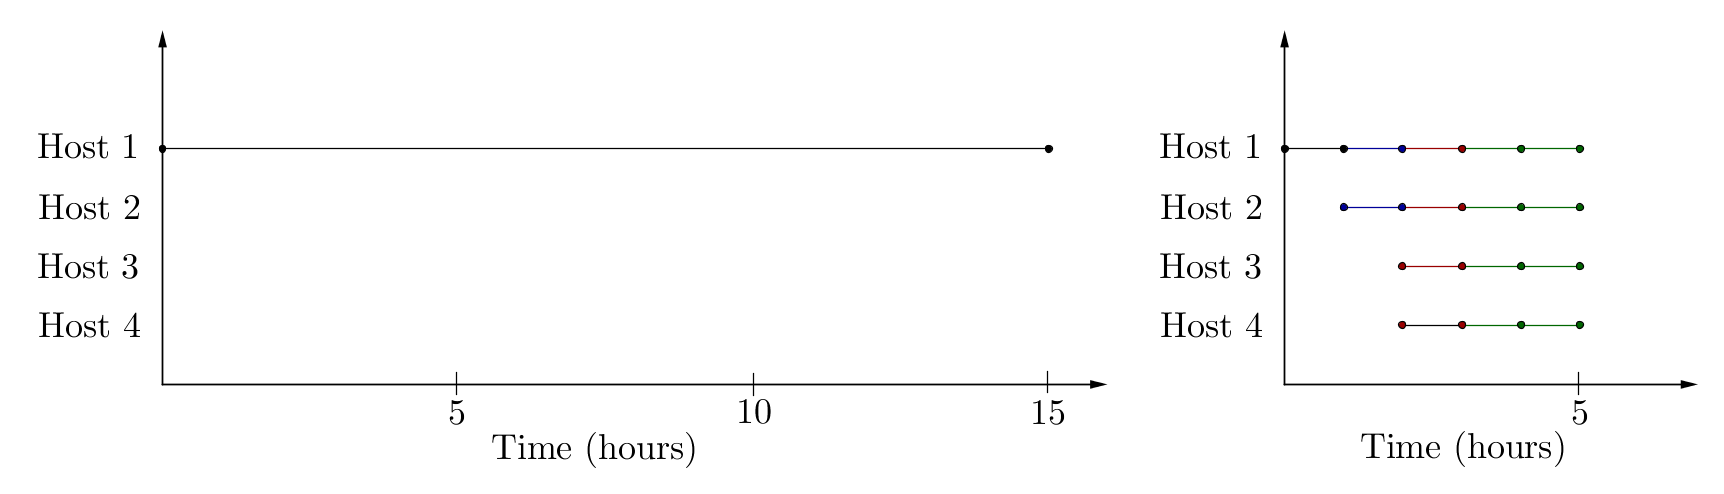
\includegraphics[width=15.5cm]{images/splits}
\caption{A visual representation of the work performed by four hosts to complete a workunit of 15 hours, firstly under the basic scheduling rules in \S\ref{5grid} and secondly under the splitting and recycling policy of \S\ref{5gen}. Every line segment represents a single workunit, and workunits of the same colour were created during the same round of recycling.} \label{fig:splits}
\end{figure}

Figure \ref{fig:splits} shows what the impact of this would be in a hypothetical scenario with a workunit of 15 hours where four hosts are available and the length of a workunit is restricted to one hour before recycling. It is clear that the workunit will be completed much earlier if this policy is implemented, and also that it leads to a much more efficient utilization   of the available resources. The policy was also tested on the ninth node on level 0 of the enumeration tree of 3-MOLS of order 8, since this was the node on level 0 with the largest subtree. The details of the resulting enumeration, with a redundancy factor of 2, may be seen in Table \ref{839splits}. Note that the length of the longest workunit is approximately 80 minutes, compared to the more than 37 hours that the serial enumeration took and that there was very little overhead involved in handling multiple workunits, the average computation time of $134\,977.7$ seconds compares quite favourably to the serial enumeration time of $132\,480.7$ seconds. Furthermore, the computation is divided much more evenly between hosts under the recycling policy and the final result was received approximately 21 hours after the creation of the first workunit, a significant improvement on the 38 hours that the simple enumeration took.
\begin{table}[t]
 \centering
 \caption{A comparison of the enumeration of the ninth node on level 0 of the enumeration tree for the ernumeration of 3-MOLS of order 9 under different workunit-management policies.}
\begin{tabular}{llrrrrrrrr}
\toprule
Policy & Host   & Valid   & Credit   & CPU Time& Smallest wu & Largest wu& Avg. wu\\ \midrule
\S\ref{5grid} & 3 & 2 & $1\,868.22$ & $265\,818.7$ & $132\,480.7$ &$133\,338$& $132\,909.35$\\ \midrule
\multirow{5}{2cm}{\S\ref{5gen}} &$1$   & $46$  & $1\,377.08$ & $111\,586.0$ & $0.01$ & $3\,856.28$ & $2\,425.78$ \\
&$3$   & $24$  & $516.17$ & $50\,022.0$ & $0.01$ & $4\,570.62$ & $2\,084.25$ \\
&$5$   & $2$   & $15.76$ & $1\,174.1$ & $585.52$ & $588.54$ & $587.03$ \\
&$6$   & $34$  & $1\,887.41$ & $107\,173.4$ & $0.01$ & $4\,266.06$ & $3\,152.16$ \\ \cmidrule{2-8}
& Total   & $106$  & $3\,796.43$& $269\,955.4$ & $0.01$& $4\,570.62$ & $2\,546.75$\\ \bottomrule
\end{tabular}\vspace*{-.4cm}
\label{839splits}
\end{table}

In the implementation of this policy it was decided to only split workunits when the remaining number of unsent results was less the total that could potentially be assigned to the hosts if they all requested work simultaneously, in other words, whenever there was a chance of under-utilizing some of the hosts. This prevented a big backlog of workunits building up due to the incessant splitting of workunits. 

The workunit-management policies described here, namely the recycling and dynamic splitting of workunits, were implemented on the BOINC project server on the form of a Python \cite{python} script which periodically executes after the assimilator moves all the completed results to a folder. Every completed result which is marked as a checkpoint may be split, depending on the current level of unassigned workunits, and is recycled as a new workunit. Completed workunits  are moved away to different folder where the current state of the tree will be updated. The pseudocode for this script is given in Algorithm \ref{alg:split}.
 \begin{algorithm}[htb]
 %\SetKwFor{If}{if}{then}{}
\SetKwInOut{Input}{input}\SetKwInOut{Output}{output} 
\Input{A list, $\mathcal{L}$, of received output files }
\Output{New workunits are created where needed}
 \BlankLine
\Begin{ 
\For{\emph{every output file $f$ in $\mathcal{L}$}}{
	\If{\emph{$f$ is a checkpoint}} 
		{\eIf{\emph{the number of unsent results is less than 8 times the number of hosts}}{
			Split the remaining work into two parts and create a new workunit for each 
		}{ 
			Recycle the checkpoint file by creating a new workunit \\			
			}	 
	}Move $f$ to the a folder of completed results	 
}   
}	
\caption{Split and recycle results} \label{alg:split}% \vspace{-2.5cm}  

\end{algorithm}


\subsection{Further enumeration results and discussion}
The 3-MOLS of order 8 were enumerated through the BOINC project under these new workunit-management policies to ensure that the recycling and splitting were implemented correctly, and also so that the enumeration may be compared to previous attempts.

  \begin{table}[htb]
 \centering
 \caption{The number of results issued in each section of the enumeration tree during the distributed enumeration of 3-MOLS of order 8, along with the resulting redundancy.}
\begin{tabular}{lrrrrrrr}
\toprule
Section & Nodes on    & Workunits & \multicolumn{4}{c}{Results} & Redundancy  \\
\cmidrule(lr){4-7}
 &level 0 && Validated & Error  & Invalid & Total &($r$)      \\ \midrule 
$z_1z_2^2z_3$ & 17& 23&46&43& 0& 89&$5.2$  \\ 
$z_1z_2^1z_5$ &14&14&28&1& 2&31&$2.2$   \\ 
$z_1z_3z_4$& 5&5&10&0&0&10& $2$    \\ 
$z_1z_7$ & 9&9&18&0&0&18&$2$   \\ \midrule
Total &45 &51&102&44&2&142&$3.3$   \\ \bottomrule
\end{tabular}\vspace*{.4cm}
\label{83splitsum}
\end{table} 

\begin{table}[htb]
 \centering
 \caption{A comparison of the enumeration of the ninth node on level 0 of the enumeration tree for the ernumeration of 3-MOLS of order 9 under different workunit-management policies.}
\begin{tabular}{lrrrrrrr}
\toprule
Host & Errors & Valid & Invalid   & CPU Time& Smallest wu & Largest wu& Avg. wu\\ \midrule
$1$ & $0$ & $227$ & $0$   & $526\,923.4$ & $0.01$ & $3\,957.98$ & $2\,321.25$ \\
$3$ & $0$ & $46$ & $0$   & $143\,388.2$ & $0.01$ & $5\,077.44$ & $3\,117.14$ \\
$4$ & $0$ & $206$ & $0$   & $365\,886.1$ & $0.00$ & $3\,280.89$ & $1\,776.15$ \\
$5$ & $0$ & $186$ & $0$   & $397\,127.4$ & $0.01$ & $4\,565.33$ & $2\,135.09$ \\
$6$ & $0$ & $151$ & $0$   & $456\,265.9$ & $0.01$ & $7\,910.44$ & $3\,021.63$ \\ \midrule
Total & $0$ & $816$ & $0$  & $1\,889\,591.0$ & $0.01$ & $7\,910.44$\\ \bottomrule
\end{tabular}\vspace*{-.4cm}
\label{83splithost}
\end{table}



Compare total number of workunits, length of longest, time from start to completion etc

\section{Potential for public launch}
\subsection{Challenges arising from tests}
\subsubsection{Volunteer churn}
\subsubsection{Server capacity}
\subsection{Estimating the run-time of publicly launched projects}
\subsection{Remaining work}
\subsubsection{Cross-platform portability}
\subsubsection{Graphics}
\subsubsection{Making use of co-processors}
sldkghsdifughi
\section{Chapter summary}
